\begin{answer}
\begin{figure}[H]
    \centering
    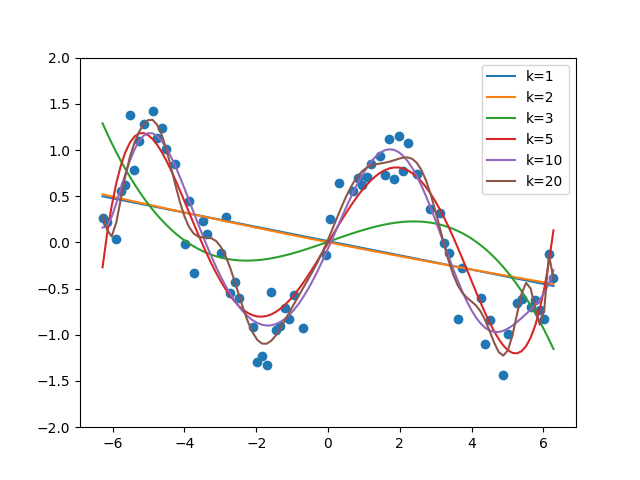
\includegraphics[width=9cm]{featuremaps/plot.png}
\end{figure}
From this plot we observe that higher degree polynomials fit the training data better. however if the axis were extended we would see how the polynomials of higher degree are very volatile and might not generalize well to other data.
\end{answer}
